\chapter{関連技術}
\label{chap:related_works}

本章では,本研究における手法を選ぶに当たって,既存の基盤手法の比較と,基盤技術として使用するRDMA(Remote Direct Memory Address)に関して述べる.

\section{オペレーティングシステム解析手段}

本セクションでは,\ref{chap:introduction}で述べた,既存のオペレーティングシステムおよびプロセスの解析技術について述べる.
コアダンプを用いた静的解析や,kgdb,VMを用いた解析に関して述べた後,その手法の一つであるlibvmiについて述べる.

\subsection{コアダンプを用いた静的解析}

コアダンプとは,

\subsection{kgdb}

\subsection{VMを用いた解析}

\subsubsection{libvmi}

\section{RDMA}

ここにRDMAの説明をかく

\begin{figure}[htbp]
    \caption{PCI Express}
    \label{fig:zentai}
    \begin{center}
        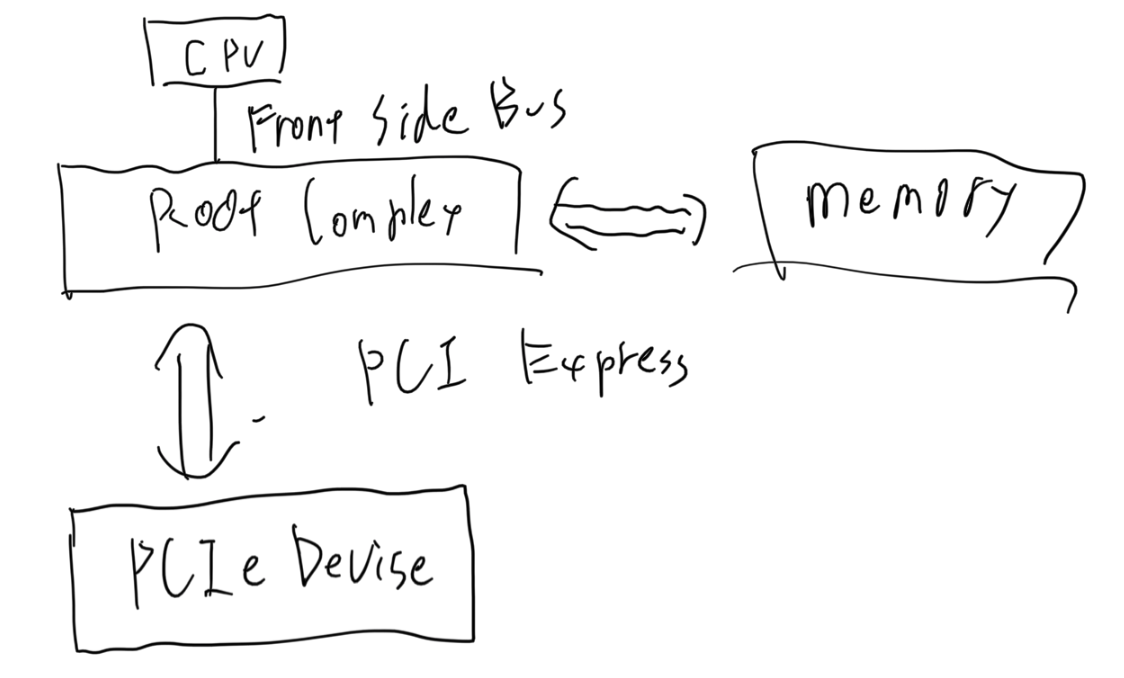
\includegraphics[bb=0 0 1000 400,width=15cm]{img/tegaki/pcie.png}
    \end{center}
\end{figure}

\subsection{InfinibandにおけるRDMA実装}
